\documentclass{manual}
\pagenumbering{gobble}

\usepackage{listings}

\title{circulator}

\begin{document}

\maketitle

\vspace*{\fill}
\begin{center}
  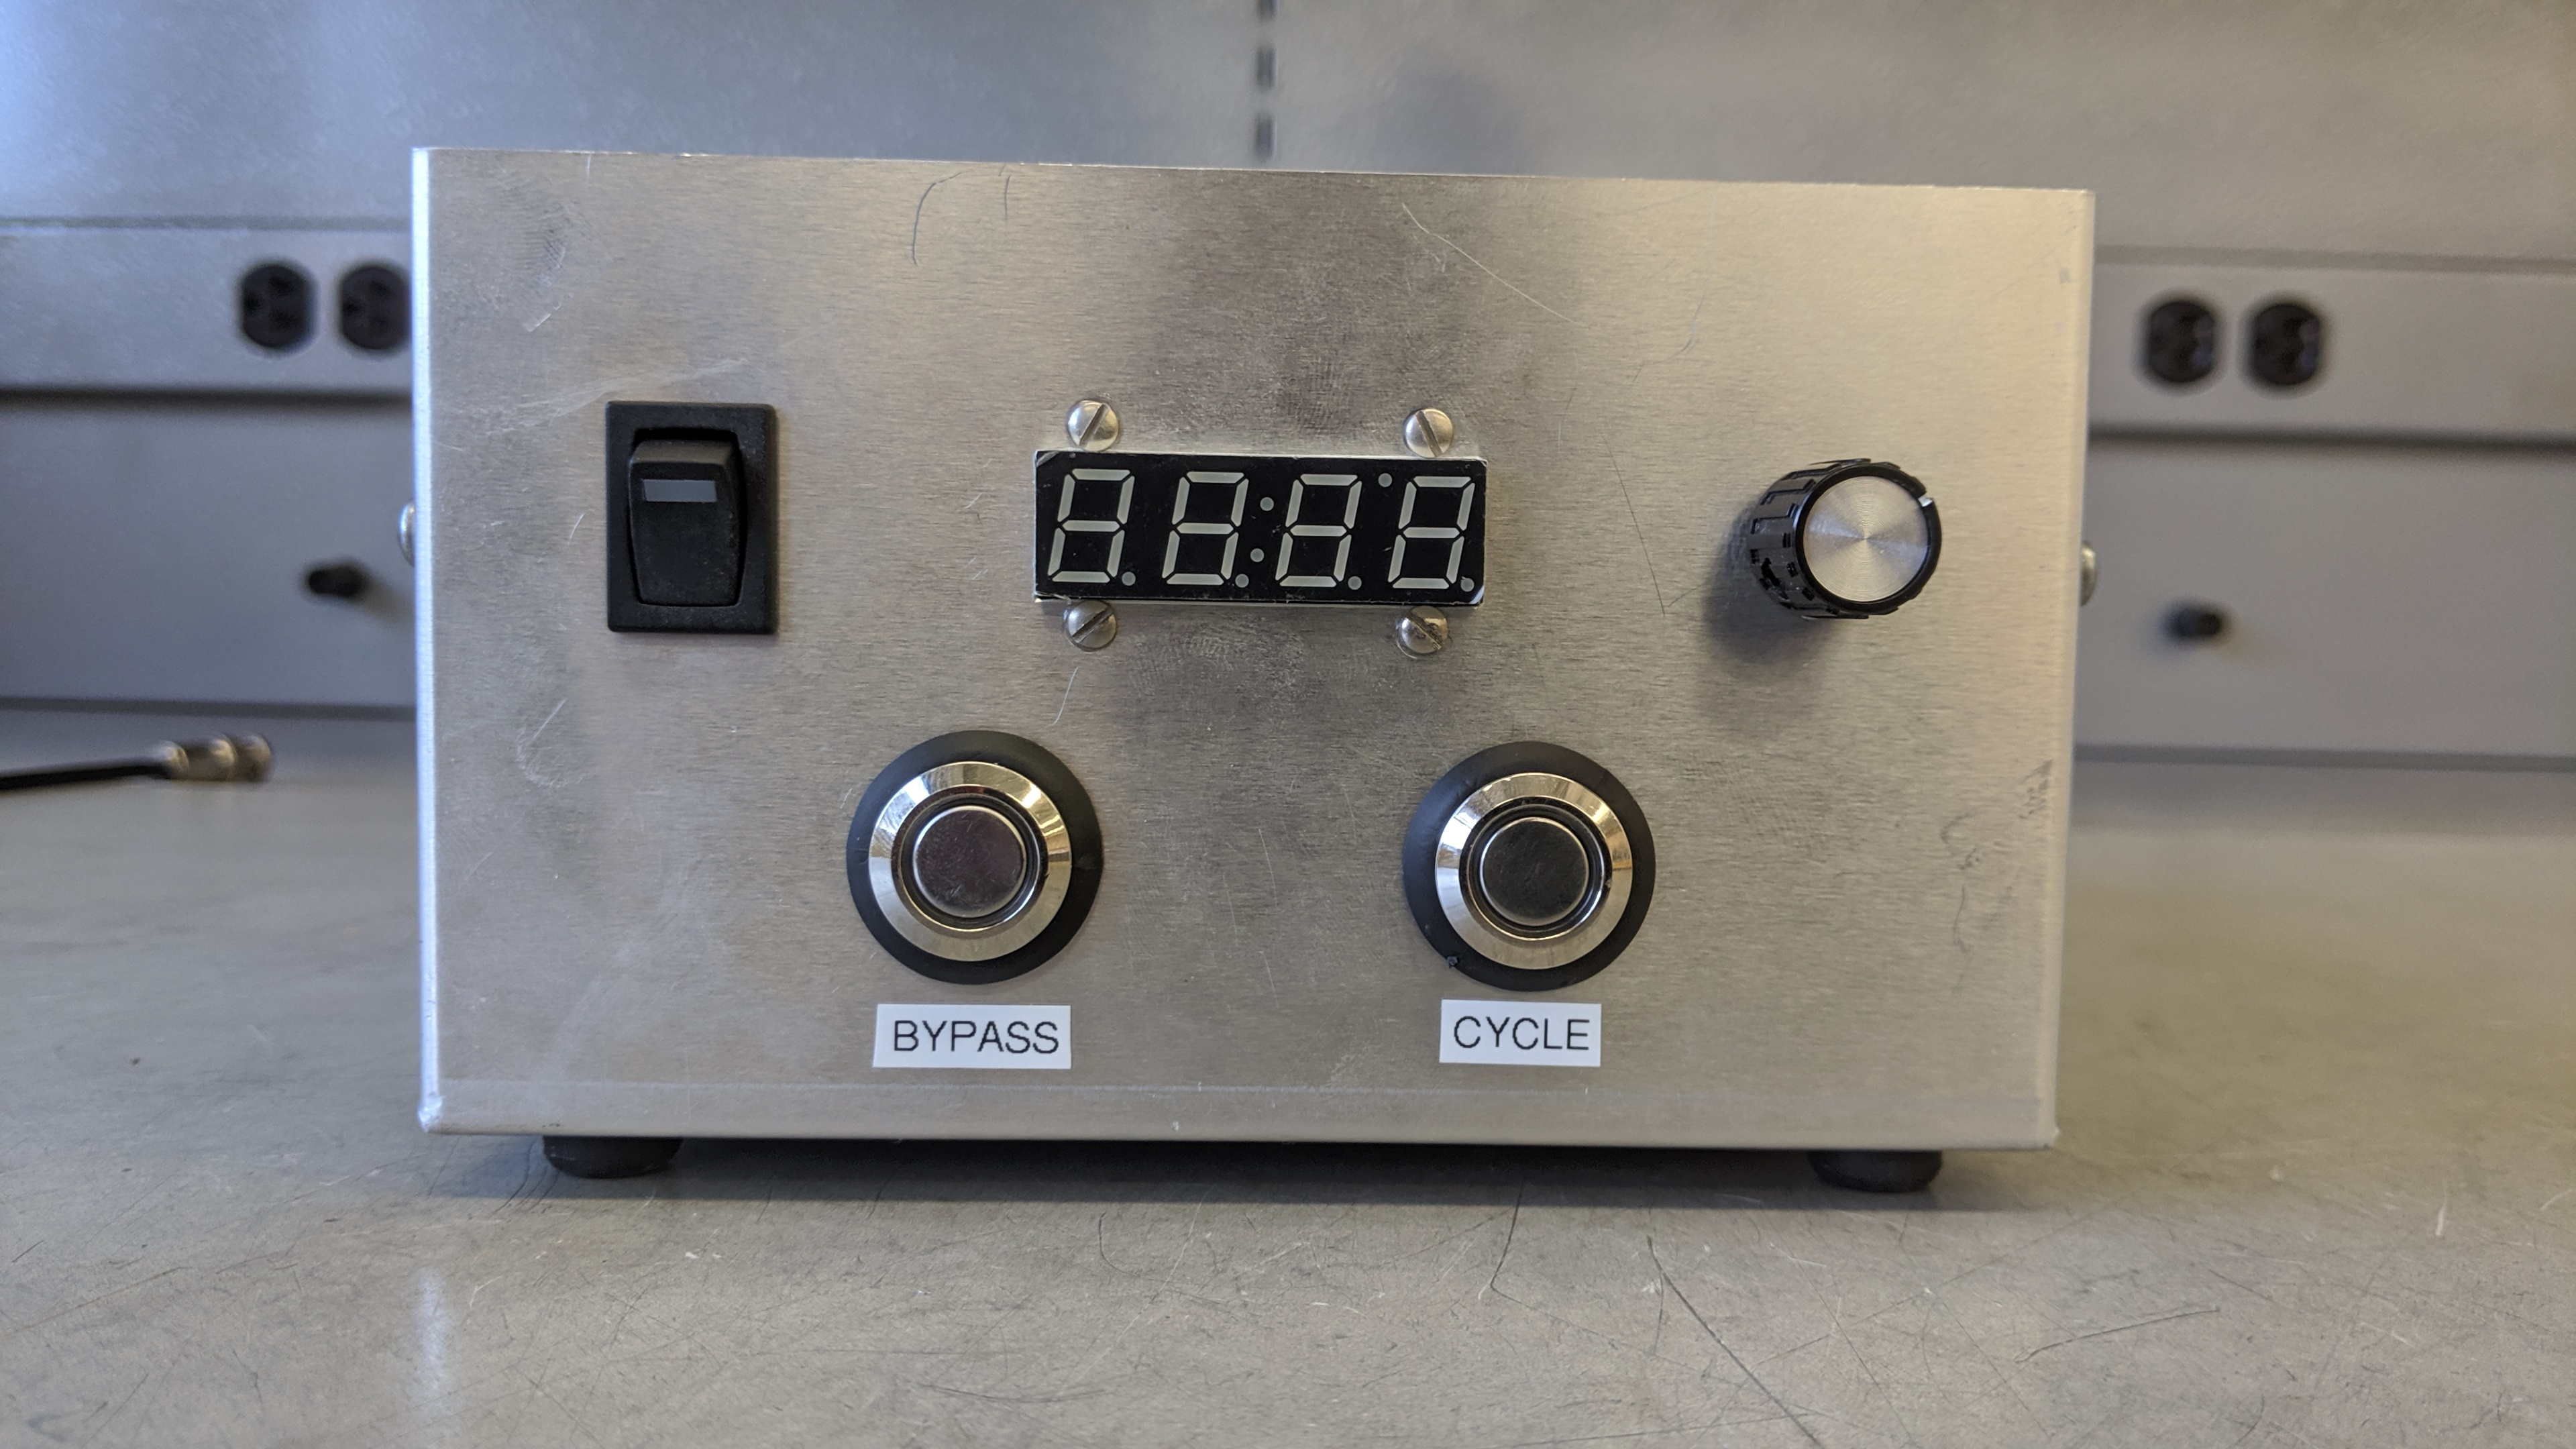
\includegraphics[width=\linewidth]{../pictures/2019-10-23_114104}
\end{center}
\vspace*{\fill}

\section{description}
\pagenumbering{arabic}

The circulator is responsible for mass transport within the WiHP-NMRR.
It consists of five solenoid valves, and two core solenoids that drive a central piston.
These fire in a certain pattern to drive gas through the WiHP-NMRR.

The circulator driver is an box of electronics that drive the seven solenoids.

\section{solenoids, cable}

\begin{center}
  \includegraphics[width=\linewidth]{./figures/solenoids}
\end{center}

The image above shows the circulator itself, with the five solenoid valves and two piston solenoids labeled.
The valves are labeled with numbers, one through five.
The piston drivers are labeled with letters, A and B.
This convention is maintained throughout this document.

Valves 1, 2 and 5 are normally closed.
Valves 3 and 4 are normally open.
The following pattern must be followed to circulate:

\begin{table}[h]
\begin{tabular}{l|ll}
  & "tick" & "tock" \\ \hline
A & energized & denergized \\
2 & energized (open) & denergized (closed) \\
4 & energized (closed) & denergized (open) \\
B & denergized & energized \\
1 & denergized (closed) & energized (open) \\
3 & denergized (open) & energized (closed)
\end{tabular}
\end{table}

On the ``tick'' step, the piston moves from B to A, pulling gas through valve 2 and pushing gas out through valve 3.
On the ``tock'' step, the piston moves from A to B, pulling gas through valve 1 and pushing gas out through valve 4.

Valve five bypasses the circulator, and is operated separately from the rest of the solenoids.
The circulator is bypassed when valve five is energized.

\clearpage

Electrically, the five valves all operate on 120 V AC.
The two piston solenoids operate at 12 V DC.
Each of the components has a separate wire controlling line (or positive) voltage within the cable.
The components share ground and neutral.
The piston solenoids are ground referenced.

The circulator is connected by a circular plastic connector, TE/AMP part numbers 206037-1 and 206036-1.
The pin designations are as follows.

\begin{table}[h]
\begin{tabular}{l|ll}
pin & color & assignment \\ \hline
1 & white & neutral \\
2 & red & valve 1 \\
3 & orange & valve 2 \\
4 & yellow & valve 3 \\
5 & blue & valve 4 \\
6 & purple & valve 5 \\
7 & & \\
8 & & \\
9 & & \\
10 & & \\
11 & & \\
12 & & \\
13 & & \\
14 & green & ground \\
15 & brown & solenoid A \\
16 & black & solenoid B
\end{tabular}
\end{table}

\section{electrical box}

\begin{center}
  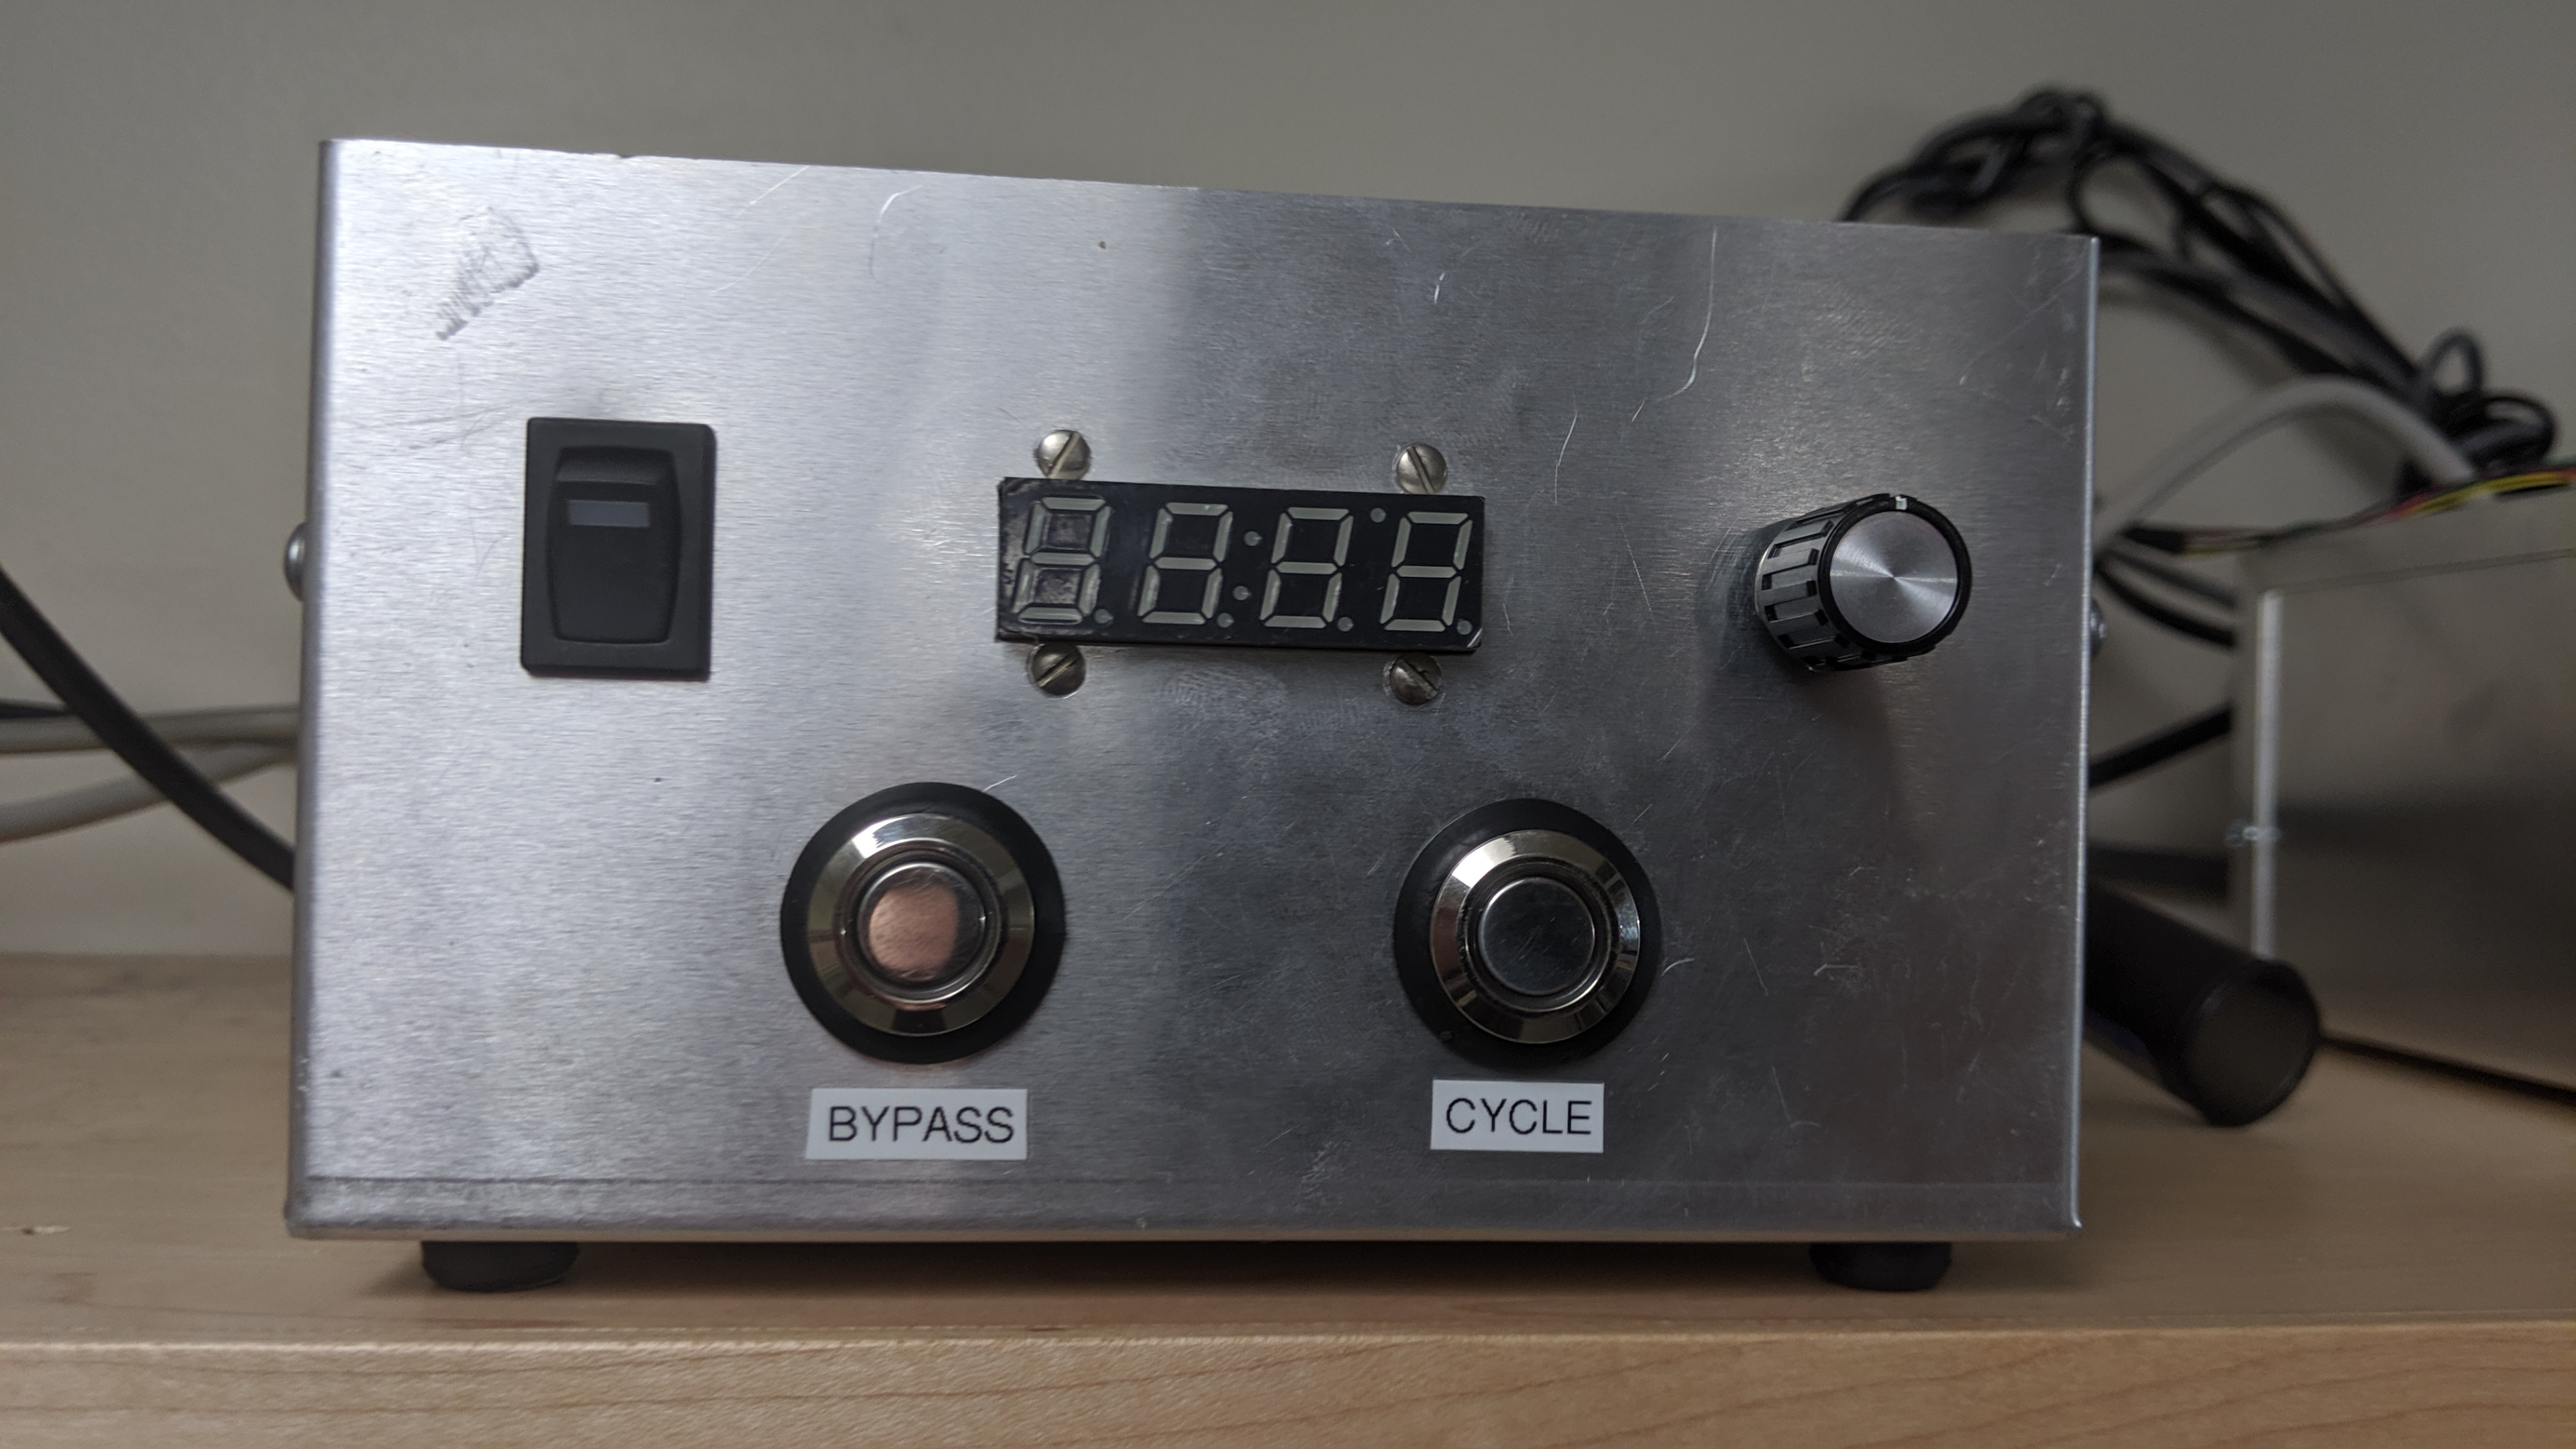
\includegraphics[width=0.75\linewidth]{../pictures/2019-10-22_162512}
\end{center}

The circulator driver controls the firing of the valves and solenoids necessary for mass transport in the WiHP-NMRR.
The image above is the front of the circulator driver box.
There is a power switch, far left.
The seven segment display in the middle shows the current circulator frequency, in Hz.
This frequency can be adjusted using the encoder knob, right.
Two buttons, one for bypass and the other for cycle, control the current status of the circulator.
Mechanically these are toggle buttons, and each toggles their corresponding state.
Each button contains an illuminated ring which will always display the current state.
These states can also be updated via TTL, as will be discussed later.

\begin{center}
  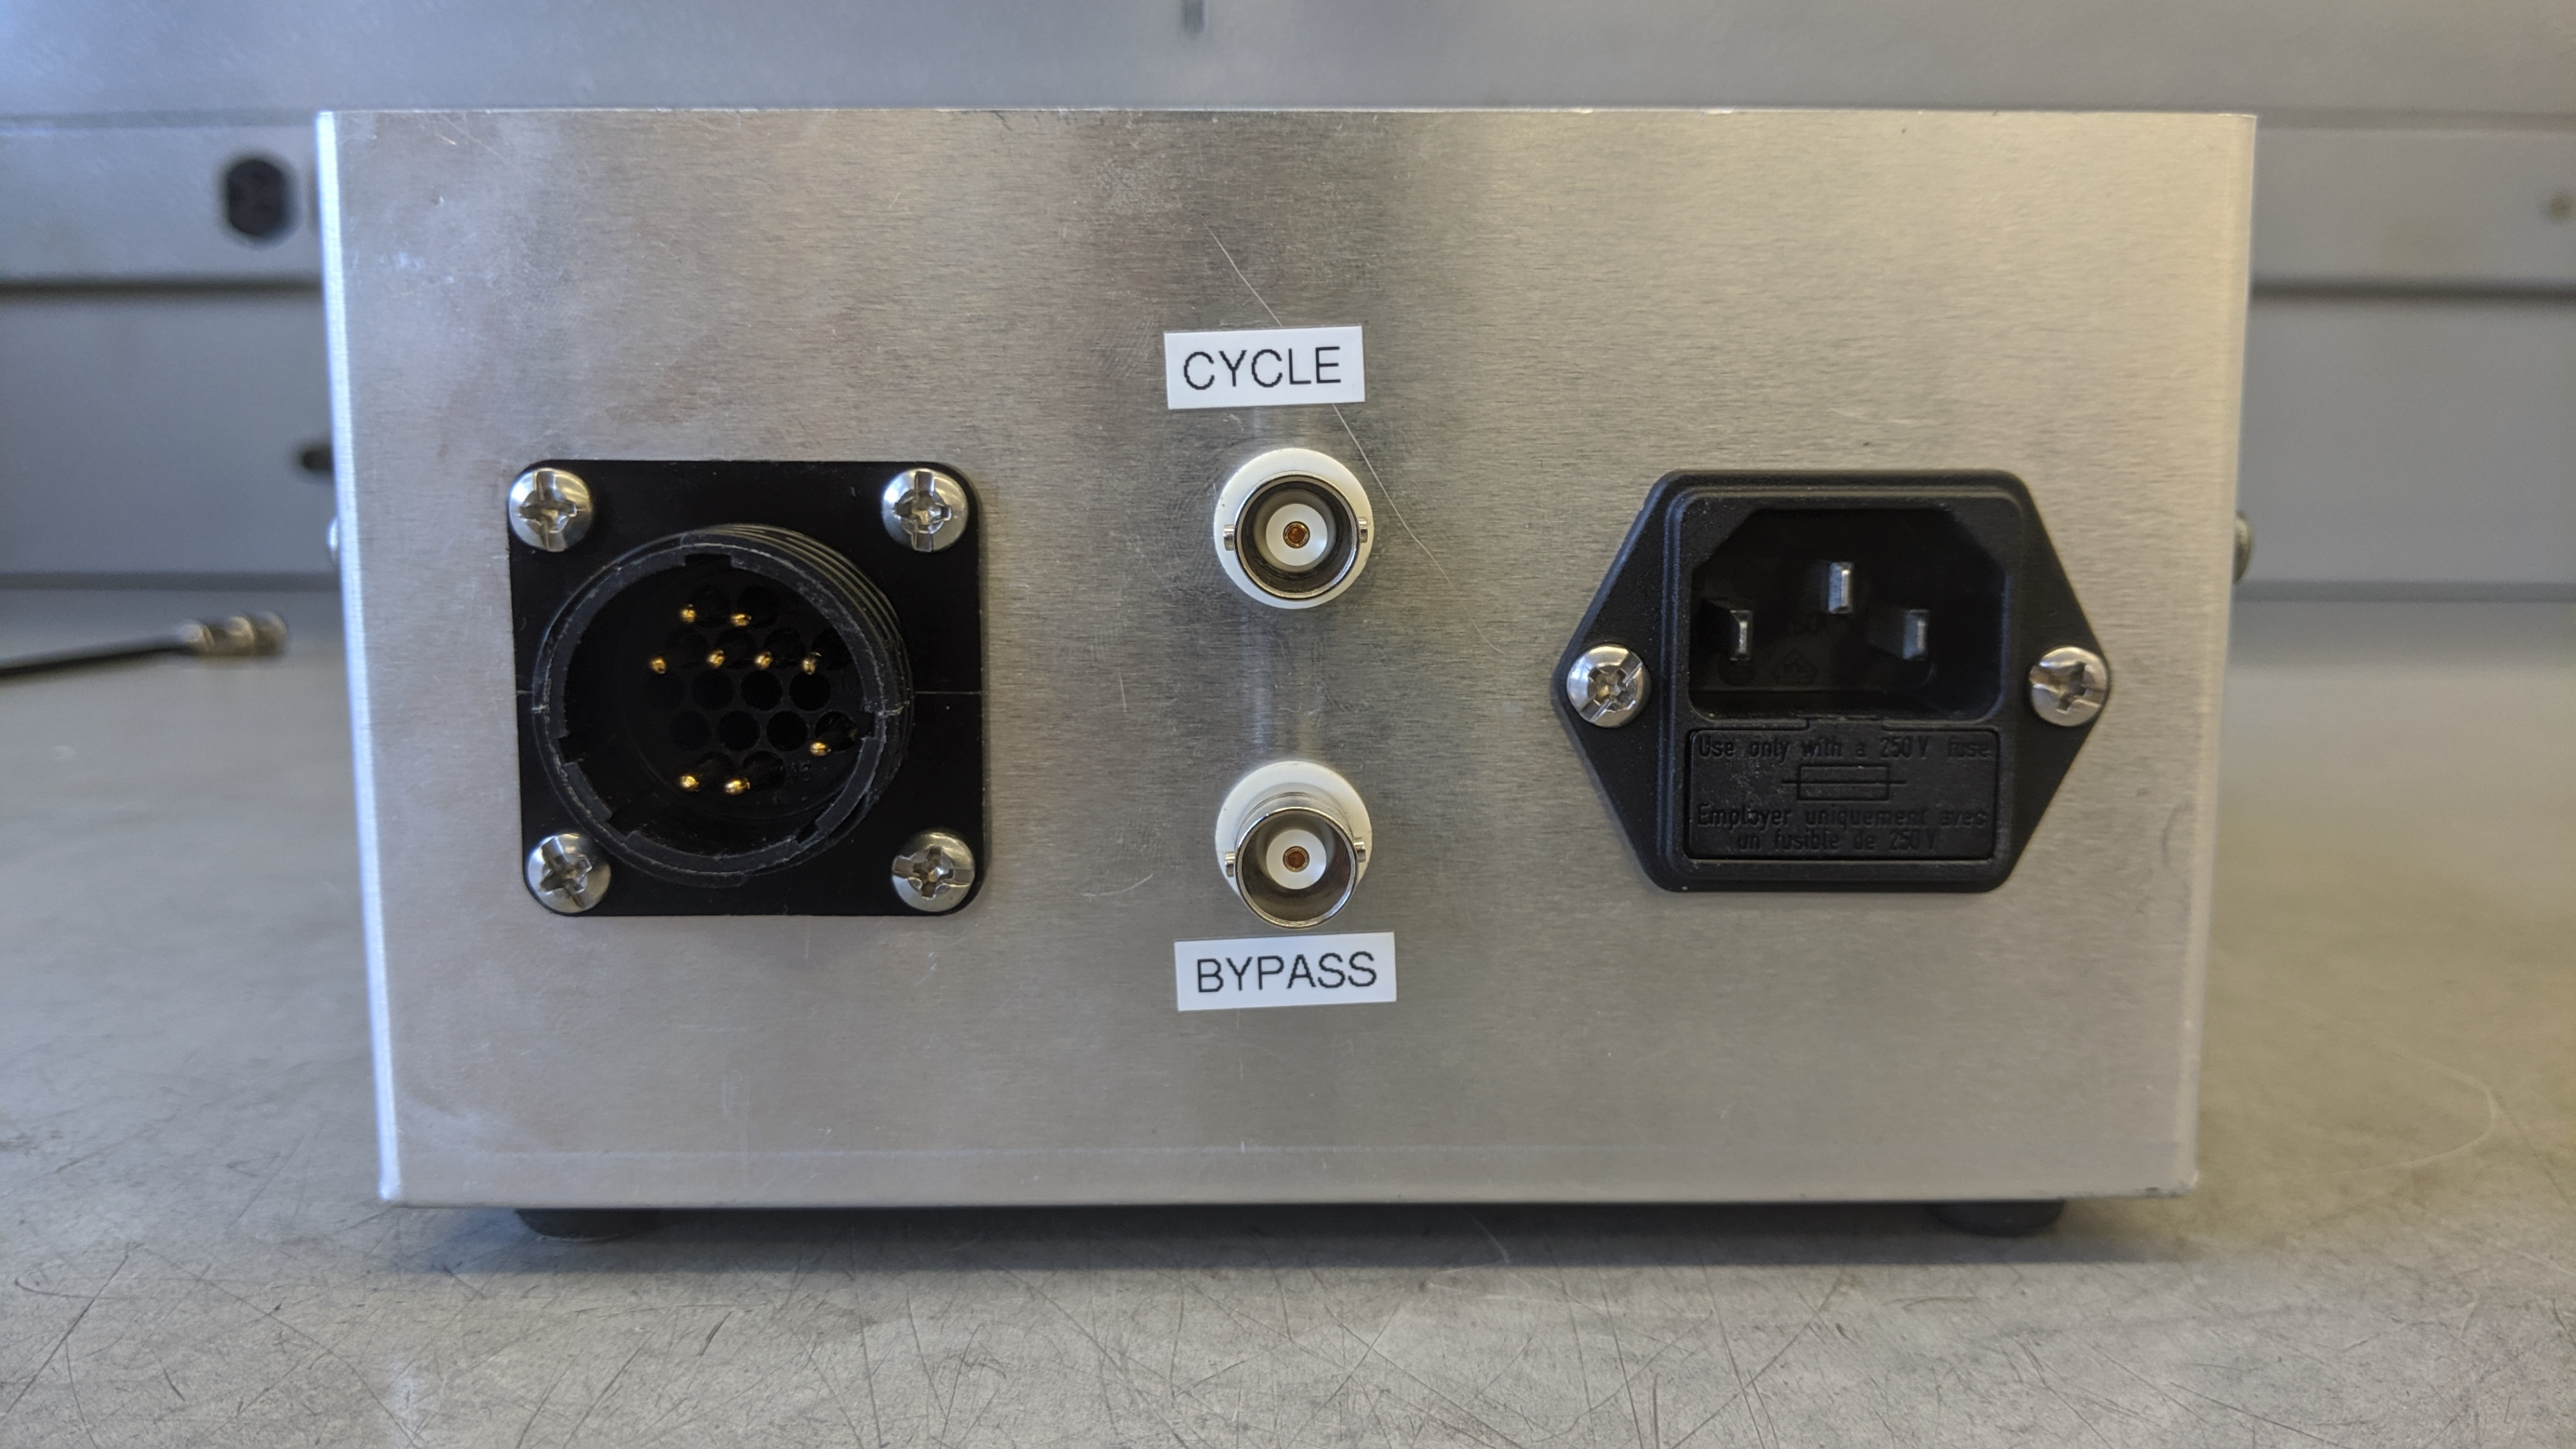
\includegraphics[width=0.75\linewidth]{../pictures/2019-10-23_114434}
\end{center}

The image above shows the rear of the circulator driver box.
There is a sixteen-pin CPC connector, left, which goes to the circulator itself.
In the middle there are two BNC inputs, cycle and bypass, which accept TTL control from the NMR.
On the right there is power input, which accepts a standard C13 connector.
The circulator operates at 120 V, and may draw up to 5 amps.
There is a fuse within the drawer immediately under the AC entry port.

\clearpage

\begin{center}
  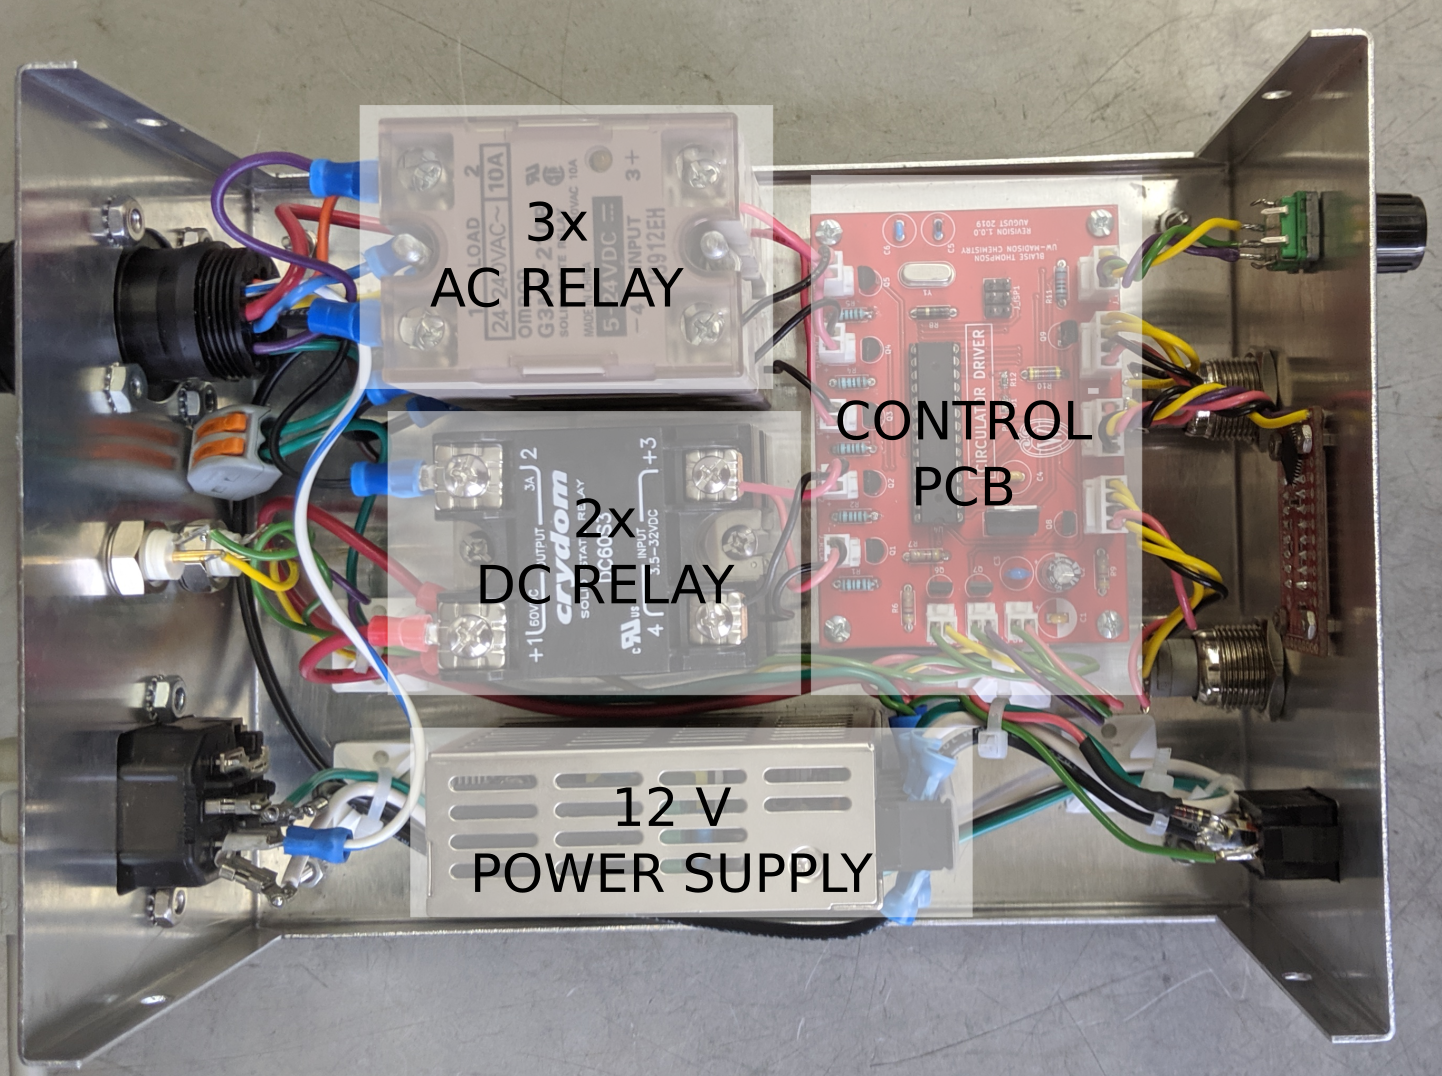
\includegraphics[width=\linewidth]{./figures/internal}
\end{center}

The image above shows the internals of the circulator driver box.
The enclosure used is 8'' x 6'' by 3.5'', Bud Industries part number CU-3009-A.
Besides the front and back panel elements, the box contains a 12 V power supply (TRACO part number  TXL 025-12S), 2 DC relays (Crydom part number DC60S3), and 3 AC relays (Omron part number G3NA-205B).
The relays and power supply make up the majority of the cost of the drive electronics.

Also contained within the enclosure is the custom control printed circuit board (PCB).
This central control board accepts power from the 12 V supply, input from the two rear-panel BNC connectors, and connects to the front panel elements and five relays.
At the core of the control board is a microcontroller with custom firmware.
These will all be discussed in the next few sections of this manual.

\section{circuit board}

\begin{center}
  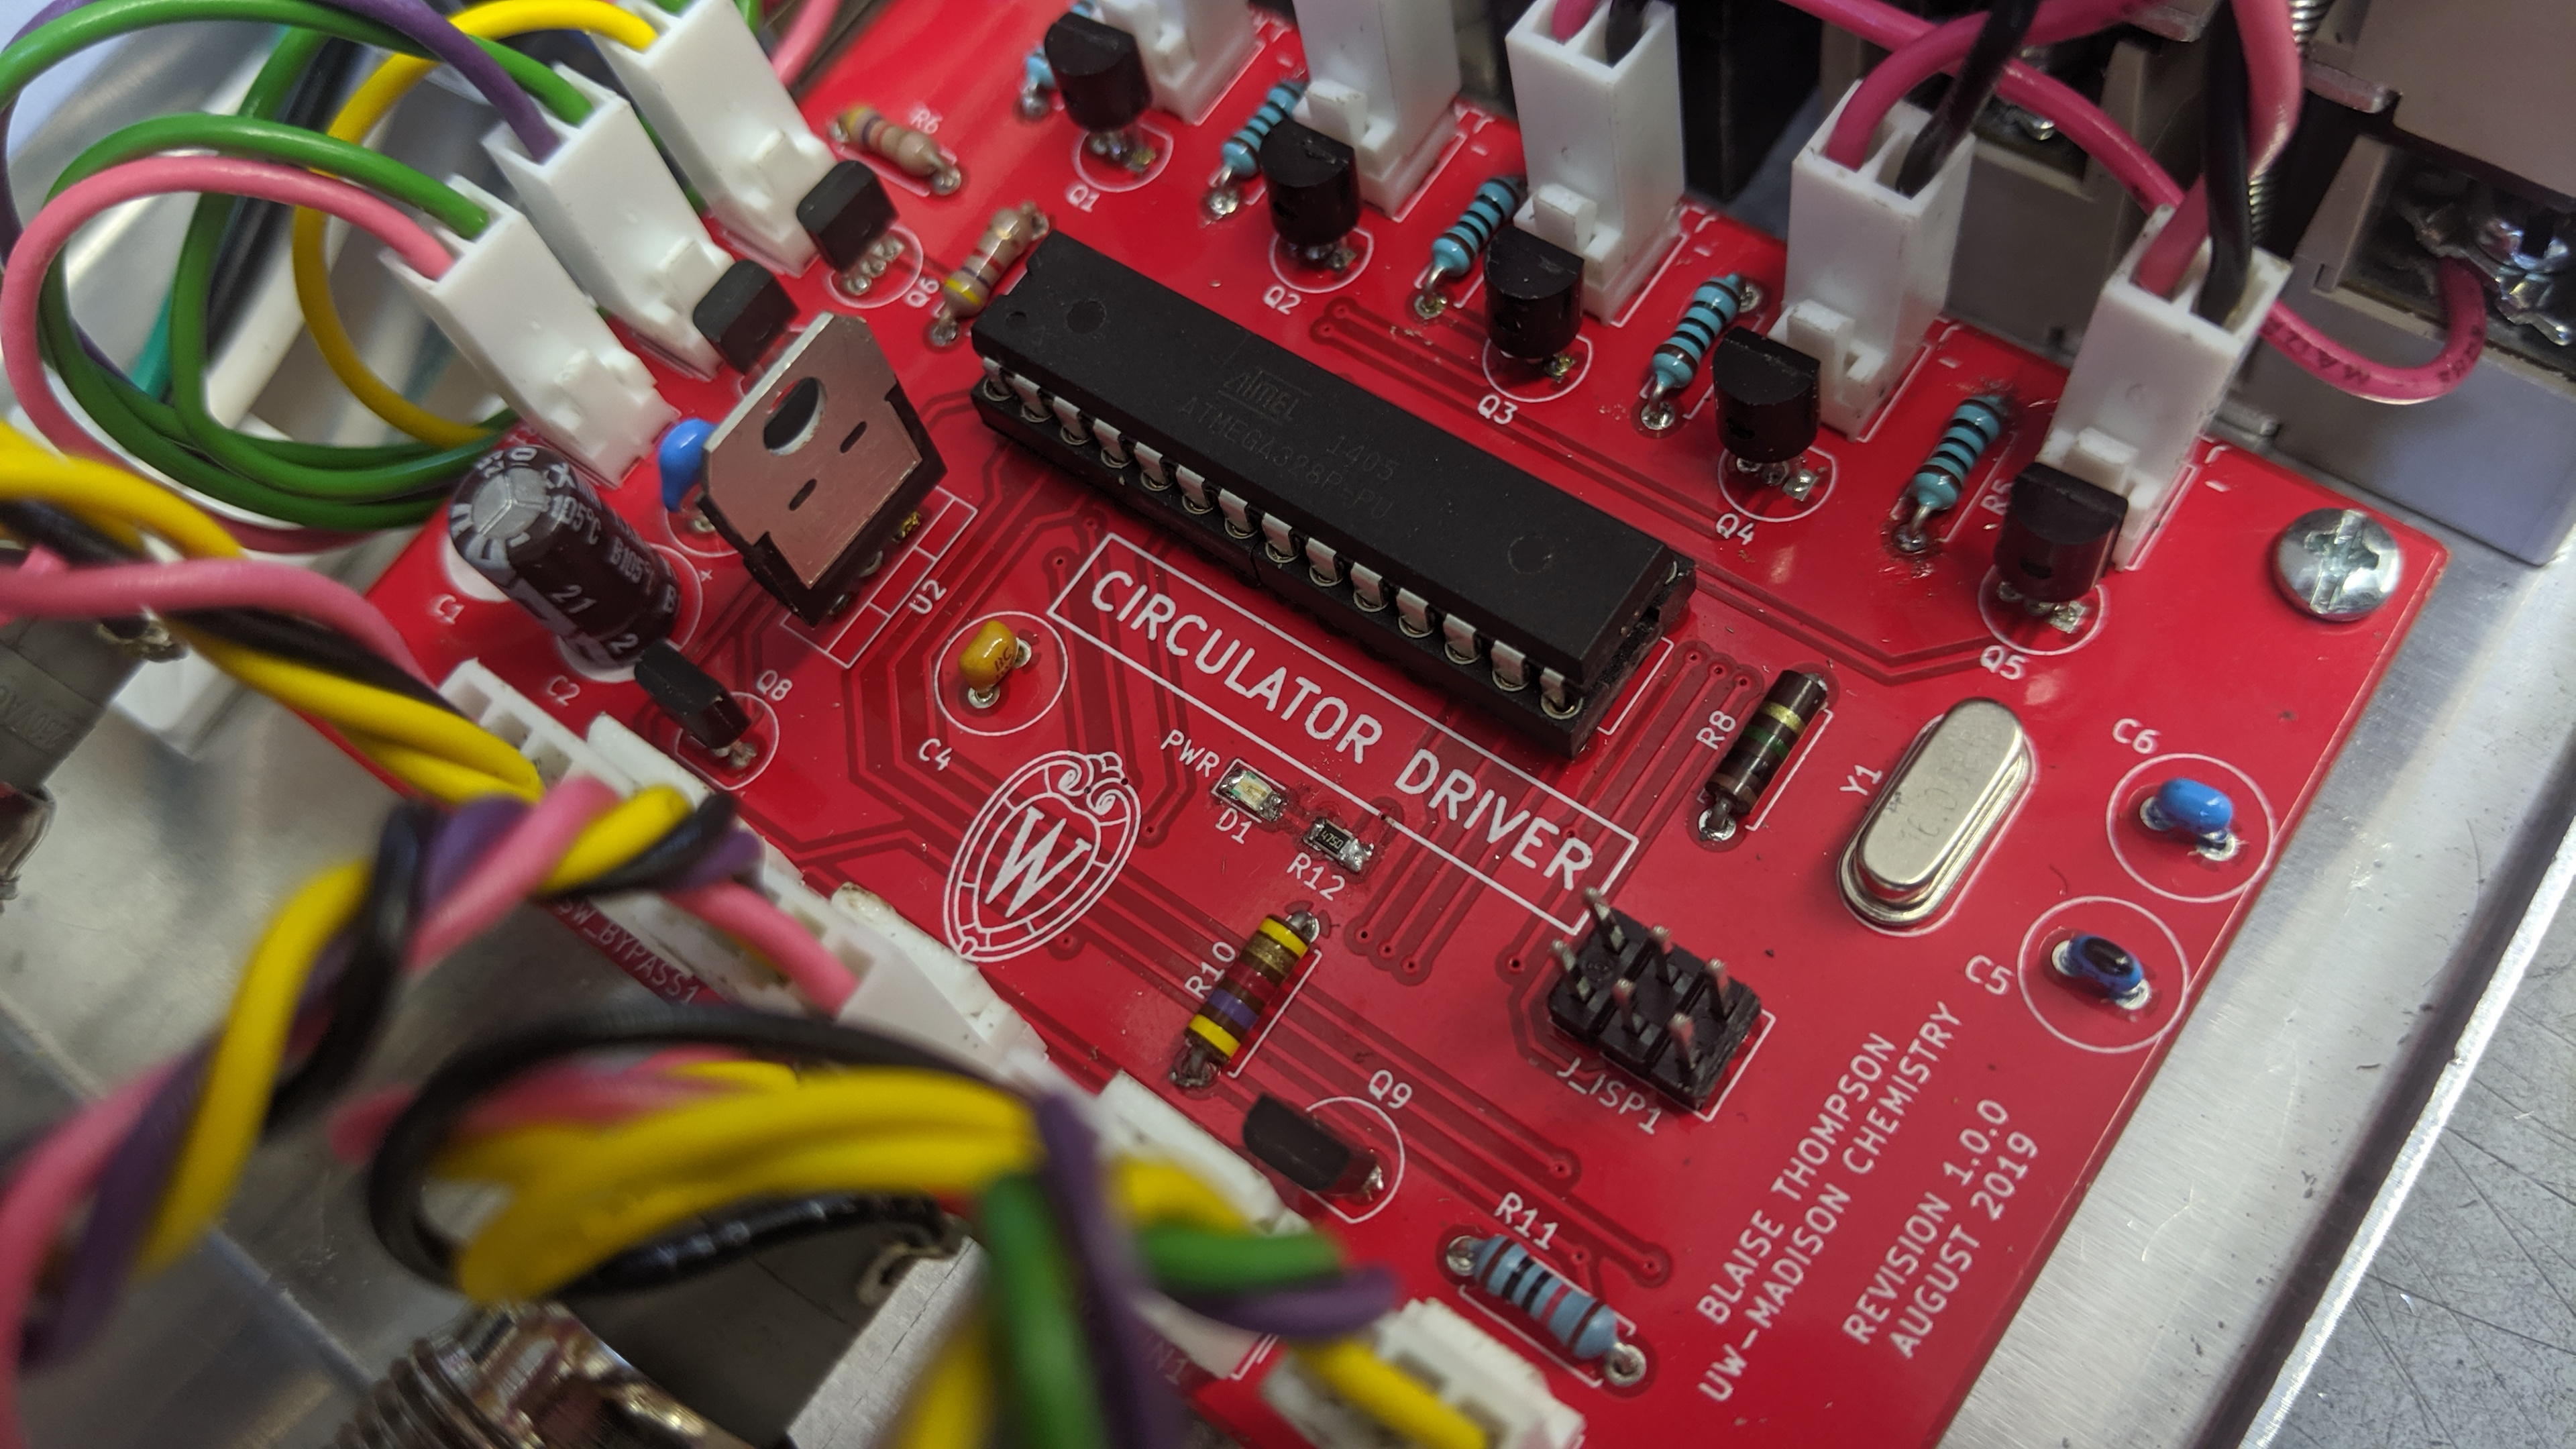
\includegraphics[width=\linewidth]{../pictures/2019-10-23_114657}
\end{center}

The following pages diagram the printed circuit board (PCB) at the heart of the circulator driver electronics.
This PCB is centered around a single microcontroller, the ATmega328.
A 16 MHz crystal supplies the clock for the microcontroller.
A standard six pin ISP header can be used to program the microcontroller in-circuit.

The microcontroller has outputs to drive five relays, each controlling the action of a small NPN transistor (2N7000) with an appropriate pull-up resistor.
These five relays drive the circulator solenoids, as described in the previous section.
The microcontroller has two TTL inputs, each buffered by a small PNP transistor (BS250) and associated pull-down resistor.

Besides these, the microcontroller has inputs for the two front-panel buttons and the front-panel encoder.
There are also outputs for the LEDs embedded within each front-panel button, and for the seven-segment display (SparkFun part number COM-11441) (driven via I2C).

The following pages contain:
\begin{enumerate}
  \item PCB schematic
  \item PCB silk screen
  \item PCB top copper layer
  \item PCB bottom copper layer
\end{enumerate}
Please note that PCB silk screen and copper representations are to-scale.

The next sections describe the microcontroller firmware and PCB components.

\includepdf[angle=0, fitpaper=true]{../PCB/pcb.pdf}
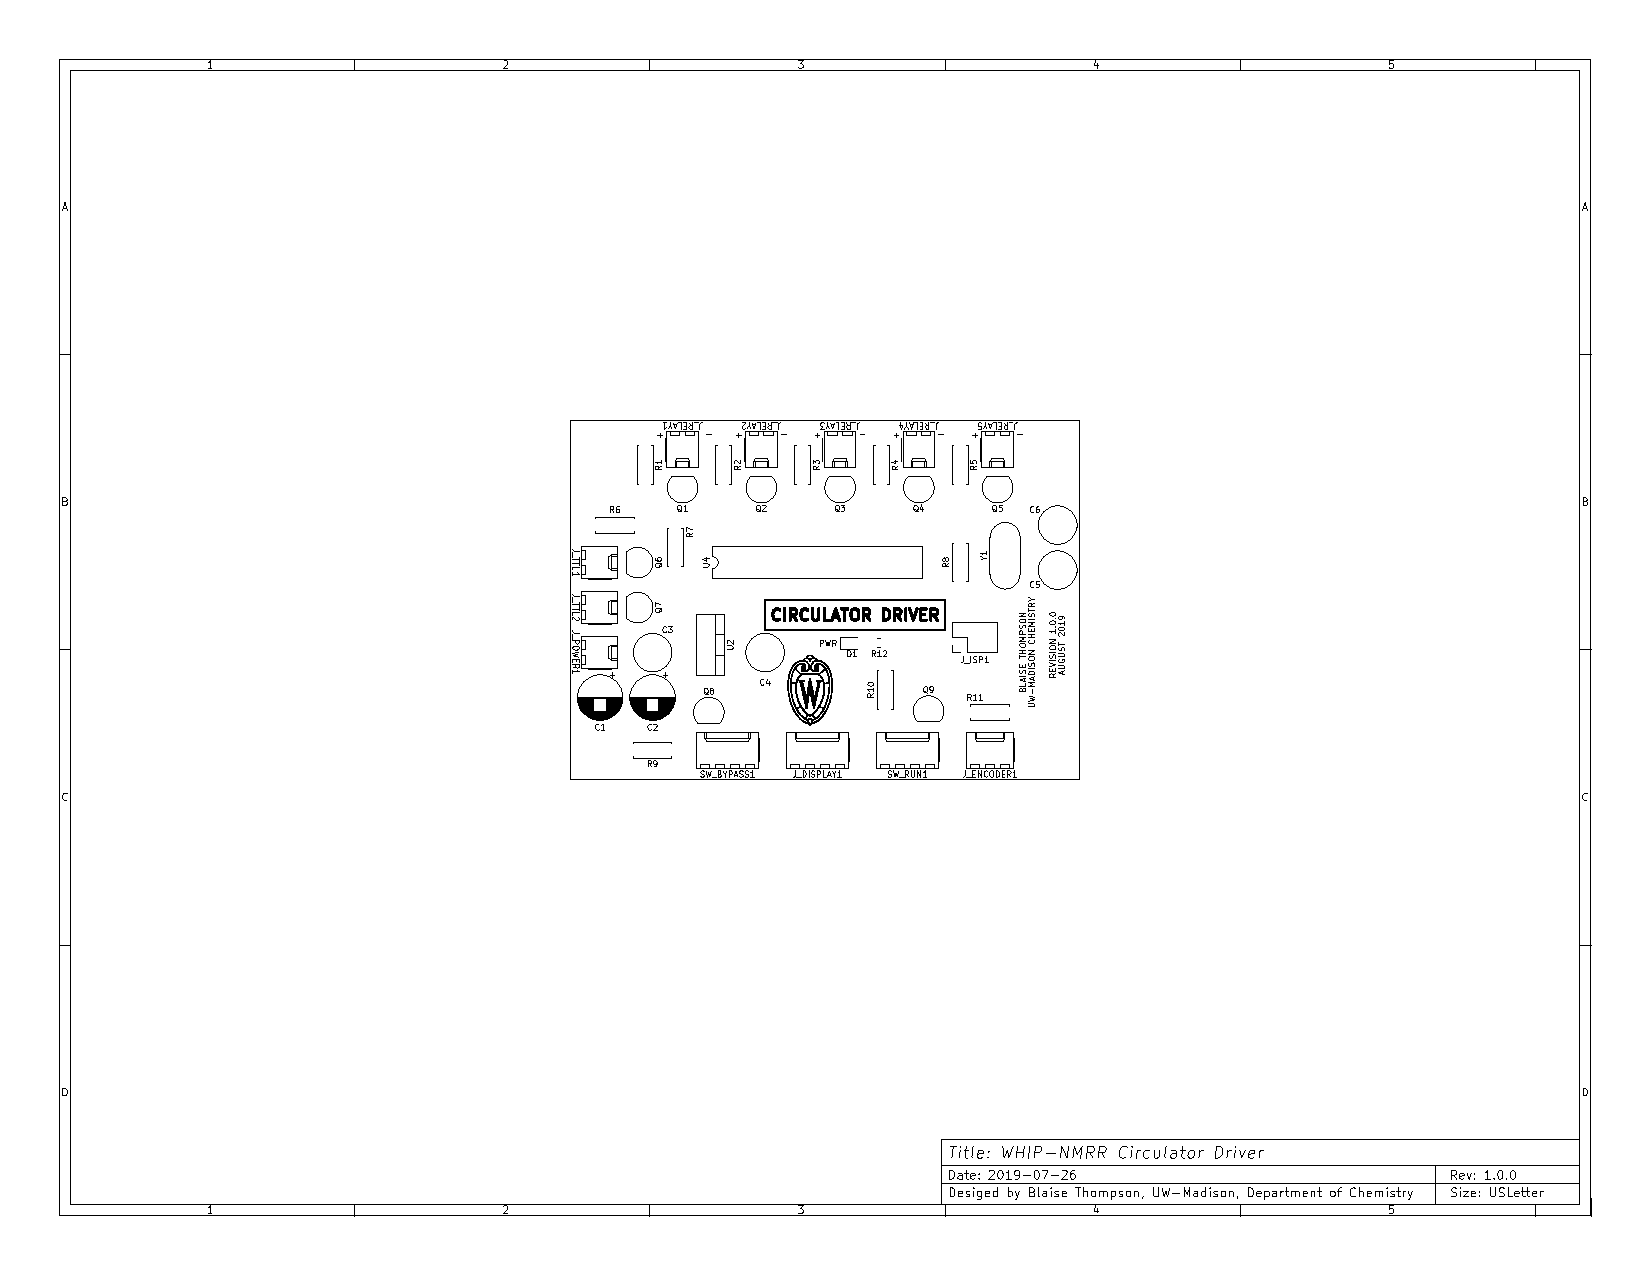
\includepdf[angle=0, fitpaper=true]{../PCB/silk.pdf}
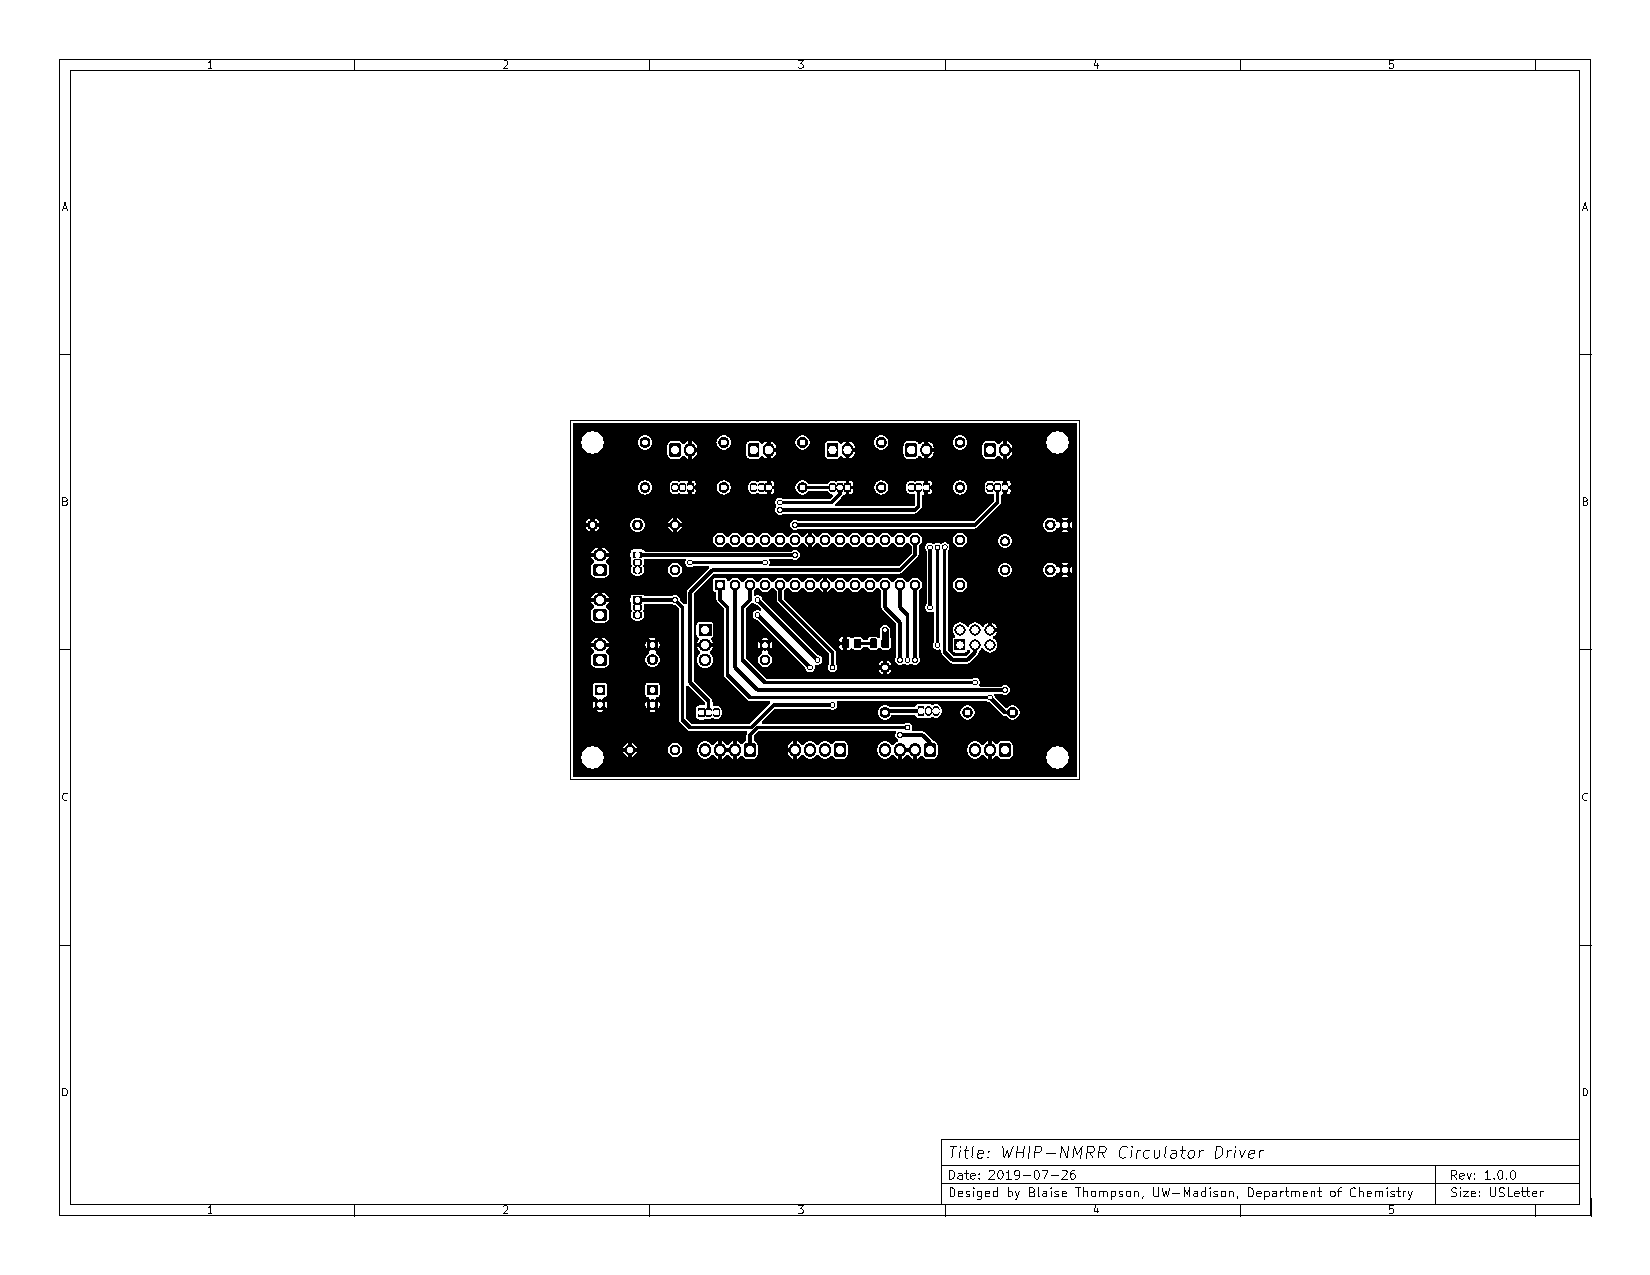
\includepdf[angle=0, fitpaper=true]{../PCB/front.pdf}
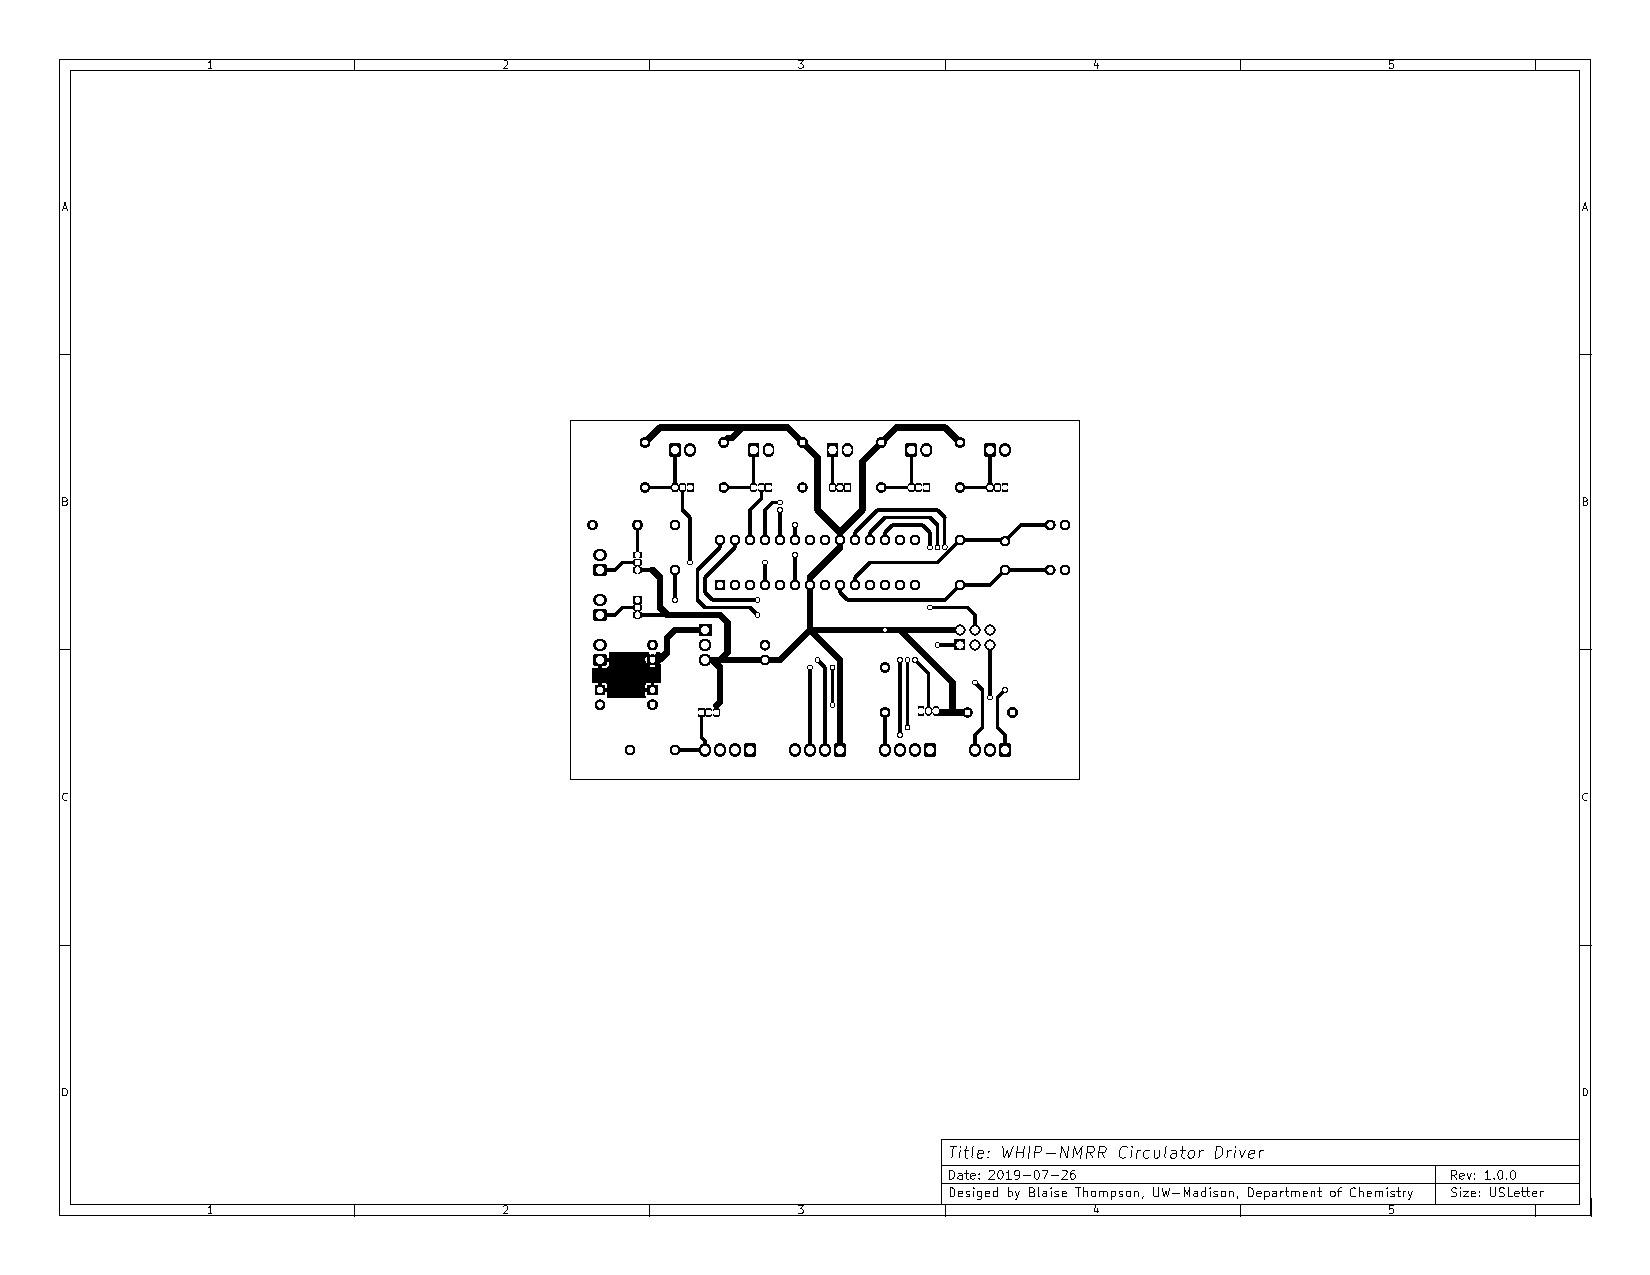
\includepdf[angle=0, fitpaper=true]{../PCB/back.pdf}

\section{firmware}

The following pages contain the raw source-code running on the embedded Atmega328 microcontroller.

\vspace{10pt}
\hrule

\lstinputlisting[language=c++]{../firmware/firmware.ino}

\section{BOM}

The following is an INCOMPLETE bill of materials for the circulator.
Trivial components like screws and resistors have been excluded.

\begin{tabular}{lrrrrl}
item & part & rate & count & total & comment\\
\hline
AC relay & G3NA-205B & 27.00 & 3 & 81.00 & \\
DC relay & DC60S3 & 21.00 & 2 & 42.00 & \\
12 V power supply & TXL 025-12S & 37.00 & 1 & 37.00 & \\
enclosure & CU-3009-A & 16.00 & 1 & 16.00 & \\
CPC pin & 66103-4 & 0.75 & 20 & 15.00 & \\
CPC socket & 1-66105-9 & 0.75 & 20 & 15.00 & \\
CPC plug & 206037-1 & 6.00 & 2 & 12.00 & \\
CPC socket & 206036-1 & 5.00 & 2 & 10.00 & \\
BNC jack & 031-10-RFXG1 & 3.00 & 2 & 6.00 & \\
AC entry & 6200-2300 & 6.00 & 1 & 5.00 & \\
16 MHz xtal & HC-49/U-S16000000ABJB & 1.00 & 1 & 1.00 & \\
header, 2 pin & 22-23-2021 & 0.25 & 8 & 2.00 & \\
header, 4 pin & 22-23-2041 & 0.50 & 3 & 1.50 & \\
header, 3 pin & 22-23-2031 & 0.25 & 1 & 0.25 & \\
DIP socket, 14 pin & 110-93-314-41-0010000 & 1.50 & 2 & 3.00 & \\
housing, 2 pin & 22-01-3027 & 0.25 & 8 & 2.00 & \\
housing, 3 pin & 22-01-3037 & 0.50 & 1 & 0.50 & \\
mosfet, N-channel & 2N7000 & 0.25 & 5 & 1.25 & \\
fuse, 1 A fast &  & 1.00 & 2 & 2.00 & \\
ring terminal, \#6, 14-16 AWG & 34158 & 0.50 & 10 & 5.00 & \\
capacitor, 33 nF & FG14X7R1H334KNT06 & 0.25 & 1 & 0.25 & \\
standoff, 0.5" \#4-40 &  & 0.50 & 4 & 2.00 & \\
housing, 4 pin & 22-01-3047 & 0.50 & 3 & 1.50 & \\
capacitor, 100 uF &  & 0.25 & 1 & 0.25 & \\
regulator, 5 V & 7805 & 1.00 & 1 & 1.00 & \\
switch & R1966ABLKBLKEFGRN & 2.00 & 1 & 2.00 & \\
7 segment display & COM-11441 & 15.00 & 1 & 15.00 & \\
rotary encoder & EN11 & 1.50 & 1 & 1.50 & \\
button, illuminated &  & 2.00 & 2 & 4.00 & \\
terminal block, 2 contact & 222-412 & 0.50 & 8 & 4.00 & \\
terminal block, 3 contact & 222-413 & 0.50 & 2 & 1.00 & \\
terminal block, 5 contact & 222-415 & 0.75 & 3 & 2.25 & \\
rubber bumper & 720 & 0.25 & 4 & 1.00 & \\
\end{tabular}

\end{document}
